\documentclass{beamer}

\usepackage{listings}
\usepackage{amsmath}
\usepackage{amsfonts}
\usepackage{amssymb}
\usefonttheme{serif}


%\usepackage{multibox,fancybox}
\usepackage{epsfig}
\usepackage{graphicx,color}
\usepackage{subcaption}
\captionsetup{compatibility=false}
\usepackage{epstopdf}

\usepackage{beamerthemesplit}
\usepackage[belowskip=-15pt,aboveskip=0pt]{caption}
\usepackage{booktabs}
\usepackage{multirow}
\setbeamercovered{highly dynamic}
\usepackage{oubraces}
%\usepackage[UglyObsolete,tight,heads=LaTeX] {diagrams}
\usepackage{pifont}
\usepackage{tikz}

\usepackage{hyperref}


\usepackage{lastpage}

\newcounter{sauvegardeenumi}
\newcommand{\asuivre}{\setcounter{sauvegardeenumi}{\theenumi}}
\newcommand{\suite}{\setcounter{enumi}{\thesauvegardeenumi}}


\newcounter{saveenumi}
\newcommand{\seti}{\setcounter{saveenumi}{\value{enumi}}}
\newcommand{\conti}{\setcounter{enumi}{\value{saveenumi}}}



\addtobeamertemplate{navigation symbols}{}{%
	\usebeamerfont{footline}%
	\usebeamercolor[fg]{footline}%
	\hspace{1em}%
	\insertframenumber
}



\renewcommand{\inserttotalframenumber}{\pageref{lastslide}}

%\setbeamertemplate{caption}[numbered]
\numberwithin{figure}{section}



\graphicspath{{Figures/}{/}}
%\theoremstyle{plain}
%\newtheorem{defn}{Definition}
%\newtheorem*{claim}{Claim}



%\useoutertheme{sidebar}
%\useoutertheme{miniframes}

%
\usetheme{Boadilla}




%\usefonttheme{Serif}

%\usecolortheme{lily}

%\useoutertheme{infolines}

% Commands



\definecolor{cec1d24}{RGB}{236,29,36}
\definecolor{cffffff}{RGB}{255,255,255}

\newcommand{\cmark}{\ding{51}}
\newcommand{\ucmark}{\tikz[y=0.80pt,x=0.80pt,yscale=-0.02,xscale=0.02, inner sep=0pt, outer sep=0pt]%
  {\path[fill=cec1d24,nonzero rule] (635.8833,600.0000) .. controls
    (651.0771,599.6647) and (665.7558,591.6224) .. (673.9783,577.5525) .. controls
    (682.1001,563.3625) and (681.7384,546.6500) .. (674.5074,533.1862) --
    (378.4699,21.6487) .. controls (370.6590,8.7662) and (356.3424,0.0975) ..
    (340.1099,-0.0063) .. controls (323.6499,0.0972) and (309.3362,8.7657) ..
    (301.4862,21.6487) -- (5.4612,533.1862) .. controls (-1.7257,546.6500) and
    (-2.0877,563.3625) .. (5.9903,577.5525) .. controls (14.2570,591.6225) and
    (28.9353,599.6650) .. (44.0853,600.0000) -- (635.8853,600.0000);
    \path[fill=cffffff,nonzero rule] (340.1208,75.7875) -- (71.0683,540.8450) --
    (608.8933,540.8450) -- (340.1058,75.7950);
    \path[fill=black,nonzero rule] (303.5900,225.7800) .. controls
    (280.4500,225.7300) and (276.9200,248.1400) .. (276.8800,250.6200) .. controls
    (276.9200,262.4400) and (285.4000,277.1700) .. (309.1600,279.4100) .. controls
    (309.1600,279.4100) and (313.7700,280.0900) .. (313.6600,283.0900) .. controls
    (313.7700,285.9400) and (313.7800,284.9700) .. (312.3400,286.5300) .. controls
    (310.8500,288.2300) and (298.5500,299.6400) .. (298.3100,302.6600) .. controls
    (296.9800,316.8800) and (300.1800,335.2800) .. (303.0900,345.9400) .. controls
    (303.0900,345.9400) and (306.6000,354.7800) .. (303.8800,361.0000) .. controls
    (301.0600,367.4700) and (289.0000,397.7400) .. (288.0000,399.5600) .. controls
    (285.1300,404.8200) and (284.0000,409.1400) .. (285.8800,415.4100) .. controls
    (284.6600,416.1100) and (264.4700,428.8800) .. (264.4700,428.8800) .. controls
    (264.4700,428.8800) and (261.3500,421.5100) .. (253.5900,419.3800) .. controls
    (245.7000,417.1100) and (239.1800,418.1800) .. (232.7200,405.9100) --
    (226.8800,396.4100) .. controls (226.8800,396.4100) and (225.6700,392.9300) ..
    (219.7500,391.6200) .. controls (213.9300,390.4900) and (206.1000,388.3000) ..
    (202.8100,388.4700) .. controls (198.6100,388.8800) and (195.2200,387.7300) ..
    (189.5900,394.2800) .. controls (185.0800,399.5300) and (112.8800,524.4700) ..
    (112.8800,524.4700) -- (286.4100,524.4700) .. controls (286.4100,524.4700) and
    (290.7100,524.0000) .. (289.5900,519.9700) .. controls (288.2700,516.1900) and
    (267.3800,441.8100) .. (267.3800,441.8100) -- (291.4400,426.7500) .. controls
    (291.4400,426.7500) and (293.3600,429.9900) .. (300.4400,426.7500) .. controls
    (307.3800,423.4800) and (309.9700,421.7500) .. (309.9700,421.7500) .. controls
    (309.9700,421.7500) and (313.9200,421.4900) .. (313.4100,413.0300) .. controls
    (316.1700,411.3100) and (341.9700,395.0600) .. (341.9700,395.0600) .. controls
    (341.9700,395.0600) and (332.8400,417.6000) .. (331.9100,427.5600) .. controls
    (331.2100,437.4600) and (327.6900,504.1200) .. (327.6900,504.1200) .. controls
    (327.6900,504.1200) and (328.1300,509.2200) .. (324.7800,510.2200) .. controls
    (321.2800,511.1700) and (305.7200,515.5000) .. (305.7200,515.5000) .. controls
    (305.7200,515.5000) and (301.3900,516.2100) .. (301.5000,519.7200) .. controls
    (301.3900,523.0400) and (303.0200,524.3400) .. (304.9400,524.4700) .. controls
    (306.9300,524.3400) and (355.7200,524.4700) .. (355.7200,524.4700) .. controls
    (355.7200,524.4700) and (360.7100,525.0000) .. (361.5300,518.4100) .. controls
    (362.3400,511.9900) and (371.5900,445.5000) .. (371.5900,445.5000) .. controls
    (371.5900,445.5000) and (367.5700,444.4500) .. (367.6200,440.5000) .. controls
    (367.5700,436.3200) and (367.5600,433.2000) .. (368.9400,431.5000) .. controls
    (370.1600,429.9500) and (384.8300,413.0400) .. (394.8800,389.5300) .. controls
    (396.4200,386.0300) and (397.5600,389.1300) .. (397.7800,390.0600) .. controls
    (398.2100,390.7500) and (417.2800,442.6600) .. (419.4700,444.7200) .. controls
    (421.8400,446.5600) and (473.3600,488.2300) .. (474.5000,489.0900) .. controls
    (475.6400,489.8600) and (478.9100,492.1100) .. (479.0000,499.3800) .. controls
    (478.9100,506.7600) and (475.9700,512.6300) .. (473.9700,514.9700) .. controls
    (472.0500,517.1900) and (468.8000,520.4500) .. (468.6900,521.8400) .. controls
    (468.8000,523.3800) and (470.2800,524.3400) .. (471.3400,524.4700) .. controls
    (472.5600,524.3400) and (479.2500,524.3400) .. (479.8100,524.4700) .. controls
    (480.5500,524.3400) and (489.3400,525.0100) .. (495.4100,514.1900) .. controls
    (501.7300,503.5300) and (513.1200,484.3400) .. (513.1200,484.3400) .. controls
    (513.1200,484.3400) and (515.5800,480.5600) .. (512.0600,478.2500) .. controls
    (508.4000,476.0100) and (502.7100,474.7100) .. (499.3800,471.1200) .. controls
    (495.8600,467.5500) and (462.9400,429.6400) .. (462.3400,428.8800) .. controls
    (461.9600,428.3400) and (457.7100,423.7600) .. (452.2800,426.2200) .. controls
    (450.7000,424.0900) and (448.8400,421.2200) .. (448.8400,421.2200) .. controls
    (448.8400,421.2200) and (439.4600,364.4600) .. (429.5300,340.4100) .. controls
    (431.8000,339.0000) and (434.8100,336.7200) .. (434.8100,336.7200) .. controls
    (434.8100,336.7200) and (442.7200,343.5500) .. (449.3800,336.4400) .. controls
    (456.0900,329.2300) and (455.6000,329.4100) .. (454.4100,326.1600) .. controls
    (453.3200,322.9000) and (452.8300,321.9100) .. (450.4400,320.5900) .. controls
    (448.2700,319.3000) and (444.5200,315.5500) .. (444.6200,308.9700) .. controls
    (444.5200,302.5400) and (441.7400,284.8000) .. (438.5300,277.2800) .. controls
    (435.5500,269.8300) and (434.5600,261.5500) .. (422.9100,256.4400) .. controls
    (404.4800,248.2100) and (379.8000,243.3100) .. (361.8100,247.9700) .. controls
    (356.8300,249.3000) and (340.8200,261.0500) .. (339.3100,261.9700) .. controls
    (337.8900,262.6800) and (331.6400,265.2600) .. (332.1900,259.8400) .. controls
    (333.4500,247.4700) and (322.7500,225.7300) .. (303.5900,225.7800) --
    cycle(394.8800,275.9700) .. controls (394.8800,275.9700) and
    (408.4700,275.8400) .. (411.5300,276.2200) .. controls (414.3400,276.5000) and
    (416.0300,280.1900) .. (416.0300,280.1900) -- (429.0000,325.8800) --
    (424.2500,328.7800) .. controls (421.5800,323.2700) and (397.9000,287.2600) ..
    (393.0300,280.4700) .. controls (389.9100,276.1000) and (394.8800,275.9700) ..
    (394.8800,275.9700) -- cycle(331.0000,332.8100) .. controls
    (331.5700,332.7900) and (332.2200,332.9700) .. (332.7200,333.2800) .. controls
    (337.8300,336.2000) and (347.5100,344.5400) .. (355.7200,356.0000) .. controls
    (356.7000,357.3200) and (355.7200,361.2800) .. (355.7200,361.2800) --
    (348.5900,376.0600) .. controls (348.5900,376.0600) and (317.8500,395.3700) ..
    (315.5000,396.9100) .. controls (312.9600,398.3000) and (311.5500,396.9300) ..
    (313.9400,393.7500) .. controls (327.6400,375.1200) and (332.7200,353.0000) ..
    (329.5300,335.1200) .. controls (329.2600,333.4800) and (330.0500,332.8500) ..
    (331.0000,332.8100) -- cycle;}}
\newcommand{\ceil}[1]{\lceil {#1} \rceil}
\newcommand{\seqof}[3]{(#1)_{#2}^{#3}}

\newcommand{\ssa}{\text{SSA}}
\newcommand{\hyb}{\text{Hyb}}
\newcommand{\MNRM}{\text{MNRM}}
\newcommand{\TL}{\text{TL}}
\newcommand{\ML}{\text{ML}}
\newcommand{\Li}{L^{\text{int}}}
\newcommand{\Ls}{L_c^{\text{exp}}}
\newcommand{\Lc}{L_c^{\text{imp}}}


%\newcommand{\NSSA}{N_{\ssa}}
\newcommand{\NSSAKone}{N_{\ssa,K1}}
\newcommand{\NSSAKtwo}{N_{\ssa,K1'}}

%\newcommand{\NMNRMKone}{N_{\MNRM,K1}}
%\newcommand{\NMNRMKtwo}{N_{\MNRM,K2}}
%\newcommand{\NMNRMKoneC}{N_{\MNRM,K1}^{(c)}}
%\newcommand{\NMNRMKtwoC}{N_{\MNRM,K2}^{(c)}}

\newcommand{\NMNRMKone}{N_{K1}}
\newcommand{\NMNRMKtwo}{N_{K2}}
\newcommand{\NMNRMKoneC}{N_{K1}^{(c)}}
\newcommand{\NMNRMKtwoC}{N_{K2}^{(c)}}

\newcommand{\NMNRM}{N_{\MNRM}}
\newcommand{\NMNRMC}{N_{\MNRM}^{(c)}}
%\newcommand{\NMNRMP}{N_{{\MNRM}^*}}

\newcommand{\NSSAP}{N_{{\ssa}^*}}
\newcommand{\NTL}{N_{\TL}}
\newcommand{\NTLP}{N_{{\TL}^*}}
\newcommand{\NTLC}{N_{\TL}^{(c)}}
%\newcommand{\NTLF}{\dbar N_{\TL}}

\newcommand{\EE}{\mathcal{E}}

\newcommand{\WE}{\EE_I}
\newcommand{\WEC}[1]{\EE_{I,#1}}
\newcommand{\WEH}[1]{\hat \EE_{I,#1}}
\newcommand{\WSSA}{\text{Cost}_{\ssa}}
\newcommand{\WHYB}{\text{Cost}_{\hyb}}


\newcommand{\avg}[2]{\mathcal{A}\left(#1;#2\right)}
%\newcommand{\SD}[2]{\mathcal{S}(#1;#2)}
\newcommand{\svar}[2]{\mathcal{S}^2\left(#1;#2\right)}

\newcommand{\dbar}[1]{\Bar{\Bar{#1}}}

\newcommand{\ie}{\emph{i.e.}}
\newcommand{\eg}{\emph{e.g.}}
\newcommand{\cf}{\emph{cf.}}
\newcommand{\ud}{\mathrm{d}}
\newcommand{\prob}[1]{\mathrm{P}\left(#1\right)}
\newcommand{\expt}[1]{\mathrm{E}\left[#1\right]}
\newcommand{\expth}[1]{\hat{\mathrm{E}}\left[#1\right]}

\newcommand{\var}[1]{\mathrm{Var}\left[#1\right]}
\newcommand{\cov}[2]{\mathrm{Cov}\left[#1, #2\right]}
\newcommand{\norm}[1]{\left\|#1\right\|}
\newcommand{\abs}[1]{\left|#1\right|}
\newcommand{\rset}{\mathbb{R}}
\newcommand{\nset}{\mathbb{N}}
\newcommand{\zset}{\mathbb{Z}}
\newcommand{\JAC}{\mathbb{J}}
\newcommand{\one}{\mathbf{1}}
\newcommand{\poisson}[1]{\mathcal{P}\left(#1\right)}
\newcommand{\normal}[1]{\mathcal{N}\left(#1\right)}
\newcommand{\binomial}[1]{\mathcal{B}\left(#1\right)}
\newcommand{\Ordo}[1]{{\mathcal{O}}\left(#1\right)}
\newcommand{\OrdoP}[1]{{\mathcal{O}_P}\left(#1\right)}
\newcommand{\ordo}[1]{{o}\left(#1\right)}
\newcommand{\abstr}[1]{\begin{abstract}#1\end{abstract}}
\newcommand{\thx}[1]{\thanks{#1}}
\newcommand{\red}[1]{{\color{red}#1}}
\newcommand{\blue}[1]{{\color{blue}#1}}
\newcommand{\green}[1]{{\color{magenta}#1}}

\newcommand{\latt}{\mbox{$\zset_+^d$}}


%Alvaro's notations

\newcommand{\indicator}[1]{\mathbf{1}_{#1}} 

\newcommand{\PERIOD}{.}
\newcommand{\COMMA}{,}

% Removed this command since it does not work properly with spacing
%\newcommand{\ChB}{{Chernoff bound }}
\newcommand{\LP}{\left(}
\newcommand{\RP}{\right)}

\newcommand{\LPe}{\left.}
\newcommand{\RPe}{\right.}

%\newcommand{\SEP}{\biggm|}
\newcommand{\SEP}{\, \big| \,}
\newcommand{\BX}{\bar X(t)}
\newcommand{\BXi}{\bar X_i(t)}
\newcommand{\BXitau}{\bar X_i(t{+}\tau)}

\newcommand{\sj}{\sum_{j=1}^J}

\newcommand{\Qi}{Q_i(t,\tau_i)}
\newcommand{\lji}{a_j(\bar X(t))\tau_i}
\newcommand{\Yj}{Y_j\left( a_j(\bar X(t))\tau_i \right)}
\newcommand{\ldi}{\log(\delta_i)}
\newcommand{\taui}{\tau_i(s)}
\newcommand{\DEN}[1]{- a_0 \LP \bar X(t) \RP +  \sj a_j(\bar X(t))e^{-#1\, \nu_{ji}}}
\newcommand{\aj}{ a_j(\bar X(t))}

\newcommand{\anu}{\sj \aj \nu_{ji}}
%\newcommand{\anu2}{\sj \aj (\nu_{ji})^2}
\newcommand{\tsi}{\tilde{s}_i}
\newcommand{\hs}{\hat{s}}
%\newcommand{\tti1}{\tilde{t}_{i,1}} 
\newcommand{\az}{a_0(\bar X(t))}
\newcommand{\dnux}{\delta_i^{\,\nu_{ji}/{\BXi}}}

\newcommand{\bj}{b_{ji}(\bar X(t))}
\newcommand{\mE}[1]{\mathcal{E}_{#1}}
\newcommand{\mV}[1]{\mathcal{V}_{#1}}
\newcommand{\hmV}[1]{\hat{\mathcal{V}}_{#1}}

\newcommand{\orden}{\alpha}

%Pedro's notations
\newcommand{\X}[1]{\bar X(t_{#1})}
\newcommand{\ti}[1]{t_{#1}}
%\newcommand{\iff}{\Leftrightarrow}

\newcommand{\algorithmfootnote}[2][\footnotesize]{%
  \let\old@algocf@finish\@algocf@finish% Store algorithm finish macro
  \def\@algocf@finish{\old@algocf@finish% Update finish macro to insert "footnote"
    \leavevmode\rlap{\begin{minipage}{\linewidth}
    #1#2
    \end{minipage}}%
  }%
}
%new command for switch case algo
% New definitions
%\algnewcommand\algorithmicswitch{\textbf{switch}}
%\algnewcommand\algorithmiccase{\textbf{case}}
%\algnewcommand\algorithmicassert{\texttt{assert}}
%\algnewcommand\Assert[1]{\State \algorithmicassert(#1)}%
%
%% New "environments"
%\algdef{SE}[SWITCH]{Switch}{EndSwitch}[1]{\algorithmicswitch\ #1\ \algorithmicdo}{\algorithmicend\ \algorithmicswitch}%
%\algdef{SE}[CASE]{Case}{EndCase}[1]{\algorithmiccase\ #1}{\algorithmicend\ \algorithmiccase}%
%\algtext*{EndSwitch}%
%\algtext*{EndCase}%

%%% Local Variables: 
%%% mode: latex
%%% TeX-master: "main_new"
%%% End: 




%\author[Outline]{Chiheb BEN HAMMOUDA (KAUST, Saudi Arabia)
% Alvaro Moraes (KAUST, Saudi Arabia)
% Ra\'ul Tempone (KAUST, Saudi Arabia)}

\institute{\scalebox{1.5}{\insertlogo}}
\setbeamercolor{author in head/foot}{bg=black,fg=white}
\setbeamertemplate{caption}[numbered]

% footline all over the presentation
\setbeamertemplate{footline}
{
	\leavevmode
	\hspace{-0.25cm}
	\hbox{
		\begin{beamercolorbox}[wd=.2\paperwidth,ht=0.4cm,dp=1.125ex,center]{author in head/foot}%
			\usebeamerfont{title in head/foot}
			\vspace{0.05cm} Chiheb Ben Hammouda, Alvaro Moraes and Raul Tempone
			\vspace{0.05cm}
			Computer, Electrical and Mathematical Science \& Engineering Division\\ King Abdullah University of Science and Technology (KAUST), Saudi Arabia
			\hspace{.3cm}
		\end{beamercolorbox}%
		
		\begin{beamercolorbox}[wd=.6\paperwidth,ht=0.4cm,dp=1.125ex,center]{title in head/foot}%tive Radio Systems
			\usebeamerfont{author in head/foot}
			\center{\vspace{0.03cm}\title{Hierarchical Stochastic  Methods for  Option Pricing and Stochastic Reaction Networks}}
		\end{beamercolorbox}%
		
		\begin{beamercolorbox}[wd=.12\paperwidth,ht=0.4cm,dp=1.125ex,left]{author in head/foot}
			\usebeamerfont{title in head/foot}
			\center{April 2015}
		\end{beamercolorbox}
		
		\begin{beamercolorbox}[wd=.08\paperwidth,ht=0.4cm,dp=1.125ex,center]{title in head/foot}%
			\usebeamerfont{author in head/foot}
			\insertframenumber / \inserttotalframenumber
		\end{beamercolorbox}%
	}
}


\setbeamertemplate{headline}
{%
	\leavevmode%
	\begin{beamercolorbox}[wd=0.5\paperwidth,ht=5ex,dp=4ex]{section in head/foot}%
		\hbox to .5\paperwidth{\hfil\insertsectionhead\hfil}
	\end{beamercolorbox}%
	\begin{beamercolorbox}[wd=0.5\paperwidth,ht=5ex,dp=4ex]{subsection in head/foot}%
		\hbox to .5\paperwidth{\hfil \insertsubsectionhead \hfil}
	\end{beamercolorbox}%
}
\renewcommand*{\inserttotalframenumber}{\pageref{lastframe}}
%%%%%%%%%%%%%%%%%%%%%%%%%%%%%%%%%%%%%%%%%%%%%%%%%%%%%%%%%%%%%%%%%%%%%%%%%%%%%%%%%%%%%%%%%%%%%%%%%%%%%%%%%%%%%%%%%%%%%%%%%%%%%%%%%%%%%%%%%%%%%%%%%%%%%%%%%%
%%%%%%%%%%%%%%%%%%%%%%%%%%%%%%%%%%%%%%%%%%%%%%%%%%%%%%%%%%%%%%%%%%%%%%%%%%%%%%%%%%%%%%%%%%%%%%%%%%%%%%%%%%%%%%%%%%%%%%%%%%%%%%%%%%%%%%%%%%%%%%%%%%%%%%%%%%
%%%%%%%%%%%%%%%%%%%%%%%%%%%%%%%%%%%%%%%%%%%%%%%%%%%%%%%%%%%%%%%%%%%%%%%%%%%%%%%%%%%%%%%%%%%%%%%%%%%%%%%%%%%%%%%%%%%%%%%%%%%%%%%%%
%%%%%%%%%%%%%%%%%%%%%%

\title[Short title]{\centerline{Adaptive sparse  grids and quasi Monte Carlo  } \\
	\centerline{
			for option pricing under the rough Bergomi model }}


\author[Short Name (U ABC)]{%
  \texorpdfstring{%
    \begin{columns}
      \column{.5\linewidth}
      \centering
     Chiheb Ben Hammouda \\	\begin{figure}[!htb]
							
\includegraphics[scale=0.18]{kaust}
 							\end{figure}
    \end{columns}
    \vspace{12pt}
    \begin{columns}
      \column{.3\linewidth}
      \centering
      Christian Bayer \\    \begin{figure}[!htb]
							
\includegraphics[scale=0.18]{WIAS}
 							\end{figure}
      \column{.3\linewidth}
      \centering
     Ra\'ul Tempone	 \\ \begin{figure}[!htb]
							
\includegraphics[scale=0.16]{RWTH}
 							\end{figure}
    \end{columns}
 }
 {Chiheb Ben Hammouda, Christian Bayer, Ra\'ul Tempone	}
}

\date[July  2019]{3rd International Conference on
Computational Finance (ICCF2019), A Coru\~na\\ 
					8-12 July,  2019 }

%%\setbeamertemplate{caption}[numbered]
%%\frame{\titlepage}
%
%%\begin{frame}[plain]
%%	\frametitle{\centerline{Adaptive sparse  grids and quasi Monte Carlo  } \\
%%		\centerline{
%%			for option pricing under the rough Bergomi model }}
%%	
%%	\setbeamercolor{block body}{use=structure,fg=black,bg=white!30!blue}
%	
%	
%	
%	\vspace{0.3cm}
%	\begin{center}
%		Chiheb Ben Hammouda \\
%	\end{center}
%	
%	
%	\vspace{0.2cm}
%	\begin{center}	
%	\textbf{Joint work with}: Christian Bayer  \& Ra\'ul Tempone		
%	\end{center}
%	\vspace{0.1cm}
%	\begin{center}
%		\today 
%	\end{center}
%	
%		
%	\vspace{0.2cm}
%	\begin{figure}[!htb]
%		
\includegraphics[scale=0.2]{kaust.jpg}
%	\end{figure}
%	\vspace{0.2cm}
%%\end{frame}




%------------------------------
\begin{document}
\begin{frame}[plain,noframenumbering]
  \maketitle
\end{frame}

\begin{frame}[plain,noframenumbering]
	\frametitle{\centerline{Outline}}
	 \tableofcontents
\end{frame}






\section{Option Pricing under the Rough Bergomi Model: Motivation \& Challenges}
\frame[plain,noframenumbering]
{\tableofcontents[currentsection,currentsubsection]}





\begin{frame}[plain]\frametitle{\centerline{Rough volatility \cite{gatheral2018volatility}}}
		\begin{figure}
		\centering
		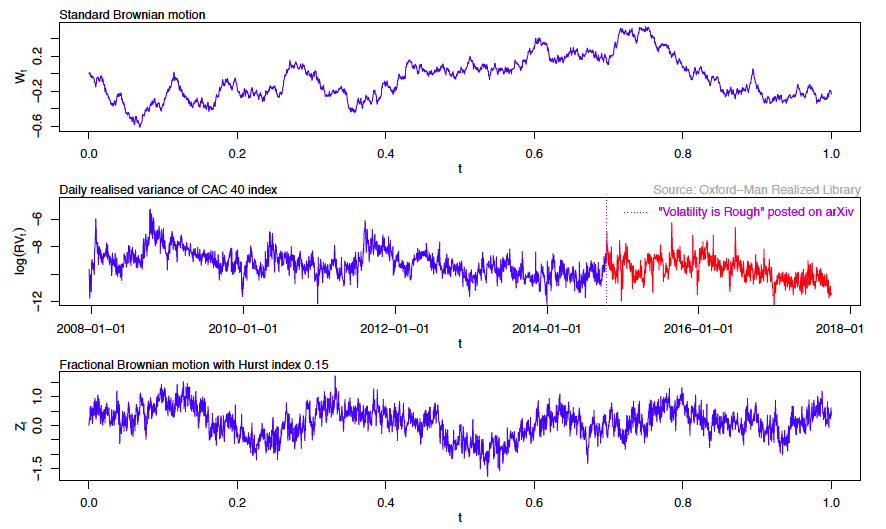
\includegraphics[scale=0.4]{vol_rough}
%		\caption{}
		\label{fig:vol_rough}
	\end{figure}
\end{frame}




\begin{frame}[plain]\frametitle{\centerline{The rough Bergomi model \cite{bayer2016pricing}}}
This model, under a pricing measure, is given by
\begin{equation}
\begin{cases}
	dS_t &= \sqrt{v_t} S_t dZ_t,\\
v_t &= \blue{\xi_0}(t) \exp\left( \blue{\eta} \widetilde{W}_t^{\blue{H}} - \frac{1}{2} \blue{\eta}^2 t^{2\blue{H}} \right),\\
	Z_t&:=\blue{\rho}	W^1_t+ \bar{\rho}W^\perp_t \equiv \blue{\rho} W^1+\sqrt{1-\blue{\rho}^2} W^\perp,
\end{cases}
\end{equation}
\begin{itemize}
	\item $(W^1,W^\perp)$: two independent standard Brownian motions
	\item $\widetilde{W}^\blue{H} $ is \red{Riemann-Liouville process},  defined by
	\begin{align*}
	\widetilde{W}_t^{\blue{H}} &= \int_0^t K^{\blue{H}}(t-s) dW_s^1, \quad t \ge 0, \\ 	K^{\blue{H}}(t-s) &= \sqrt{2\blue{H}} (t-s)^{\blue{H} - 1/2},\quad \forall \: 0 \le s \le t.
	\end{align*}
	\item $\blue{H} \in(0,1/2]$ ($H=1/2$ for Brownian motion): controls the \red{roughness} of paths, , $\blue{\rho} \in [-1,1]$  and  $\blue{\eta}>0$.
	\item $t \mapsto \blue{\xi}_0(t)$: forward variance curve, known at time $0$.
\end{itemize}
\end{frame}
\begin{frame}[plain]\frametitle{\centerline{Model challenges }}
\begin{itemize}
\item \textbf{Numerically:}
	\begin{itemize}
		\item The model is \red{non-affine} and \red{non-Markovian} $\Rightarrow$ Standard numerical methods (PDEs, characteristic functions) seem \red{inapplicable}.
		\item The only prevalent pricing method for mere
		\red{vanilla options} is \red{Monte Carlo (MC)} \cite{bayer2016pricing,bayer2017regularity,mccrickerd2018turbocharging}: still a \red{time consuming task}.
		
\item 	Discretization methods have \red{poor behavior of the strong error}, that is the convergence rate is of order of $\blue{H} \in[0,1/2]$ \cite{neuenkirch2016order} $\Rightarrow$ Variance reduction methods, such as \red{multilevel Monte Carlo (MLMC)}, are inefficient for \red{very small values} of $\blue{H}$.
	\end{itemize}

\item \textbf{Theoretically:} 
\begin{itemize}
\item No proper weak error analysis done in the rough volatility
context.
\end{itemize}
\end{itemize}

\end{frame}



\begin{frame}[plain]	
	\frametitle{\centerline{Option pricing challenges }}

	 The integration problem is  \red{challenging}

	\begin{itemize}
		\item \blue{Issue $1$:}
		Time-discretization of the rough Bergomi process (large $\blue{N}$ (number of time steps))  $\Rightarrow$ \blue{$S$}  takes values in a high-dimensional space  $\Rightarrow$ \red{Curse of dimensionality} when using numerical integration methods. 
 
		\item \blue{Issue $2$:} The payoff function \blue{$g$} is typically \red{not smooth} $\Rightarrow$ \red{low regularity}$\Rightarrow$  slow convergence of deterministic quadrature methods.
	\end{itemize}
{\fontencoding{U}\fontfamily{futs}\selectfont\char 66\relax} \red{Curse of dimensionality:} An integration error of order $\red{\varepsilon}$ requires $M$ function evaluations
\begin{equation*}
M \ge c_{\red{\varepsilon}} \blue{\bar{d}}^{-c \log \red{\varepsilon}}\COMMA
\end{equation*}
where $\blue{\bar{d}}$ depends on $\blue{d}$ and $\blue{N}$.

\end{frame}



\begin{frame}[plain]\frametitle{\centerline{Methodology }}

 We design a \red{hierarchical efficient pricing method} based on
		\begin{enumerate}
			\item \red{Analytic smoothing}  to uncover available regularity (inspired by \cite{romano1997contingent} in the context of stochastic volatility models).
			\item Approximating the option price using  \red{deterministic quadrature  methods} 
			\begin{itemize}
			\item \textbf{Adaptive sparse grids quadrature (ASGQ)}.
			\item \textbf{Quasi Monte Carlo (QMC)}.
			\end{itemize}			  
			\item Coupling our methods with \red{hierarchical transformations} $\Rightarrow$ \red{Reduce the dimension} of the problem.
			\begin{itemize}
			\item \textbf{Brownian bridges} as a path generation method.
			\item \textbf{Richardson Extrapolation} $\Rightarrow$ Faster convergence of the weak error  $\Rightarrow $ $\searrow$ number of time steps (smaller dimension).
			\end{itemize} 
		\end{enumerate} 
	
\end{frame}		


\begin{frame}[plain]\frametitle{\centerline{Simulation of the rough Bergomi dynamics}}
\textbf{\blue{Goal:}} Simulate jointly $(W_t^1, \widetilde{W}^H_t: 0 \le t \le T)$, resulting in $W^1_{t_1},\dots, W_{t_N}$ and $\widetilde{W}^H_{t_1},\dots, \widetilde{W}^H_{t_N}$ along a given grid $t_1 <\dots < t_N$ 
\begin{enumerate}
	
	\item  \textbf{Covariance based approach} \cite{bayer2016pricing}
	\begin{itemize}
	\item  Based on Cholesky decomposition of the covariance matrix  of the ($2N$)-dimensional Gaussian random vector  $W^1_{t_1},\dots, W^1_{t_N}, \widetilde{W}^H_{t_1},\dots, \widetilde{W}_{t_N}$.
	\item  \red{Exact method  but slow}.
\end{itemize}	
	\item  \textbf{The hybrid scheme} \cite{bennedsen2017hybrid} 
	\begin{itemize}
	\item Based on  \red{Euler discretization}  but crucially \red{improved by moment matching} for the singular term in the left point rule.
	\item  \red{Accurate scheme that is much faster} than the  Covariance based approach.
\end{itemize}	
	\end{enumerate}
\end{frame}



\begin{frame}[plain]\frametitle{\centerline{On the choice of the simulation scheme}}
\begin{figure}[h!]
\caption{The convergence of the weak error $\mathcal{E}_B$, using MC with $6 \times 10^6$ samples, for \red{Set $1$ parameter in Table \ref{table:Reference solution, using MC with $500$ time steps, of Call option price under rBergomi model, for different parameter constellation.}}. The upper and lower bounds are $95\%$ confidence intervals. a) With \red{the hybrid scheme}  b) With \red{the exact scheme}.}
	\centering
	\begin{subfigure}{.52\textwidth}
		\centering
		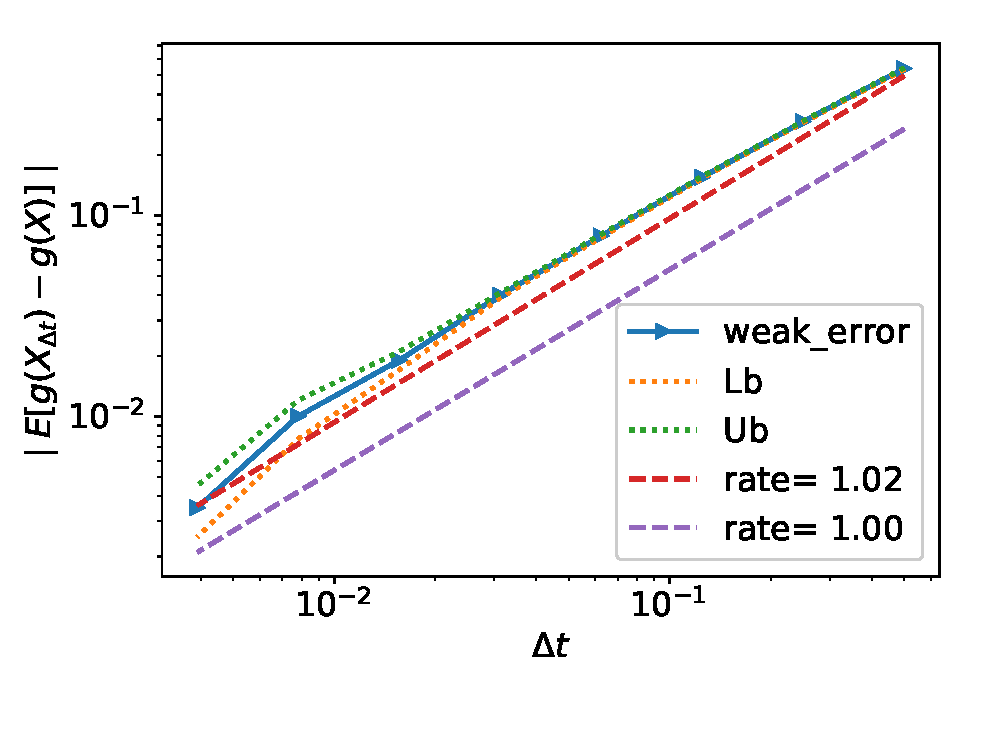
\includegraphics[width=1\linewidth]{./rBergomi_weak_error_rates/without_richardson/H_007/weak_convergence_order_Bergomi_H_007_K_1_M_4_10_6_CI_relative_hybrid_non_hierarchical_non_parallel_asymptotic}
		\caption{}
		\label{fig:set1_weak_rate_hybrid}
	\end{subfigure}%
	\begin{subfigure}{.52\textwidth}
		\centering
		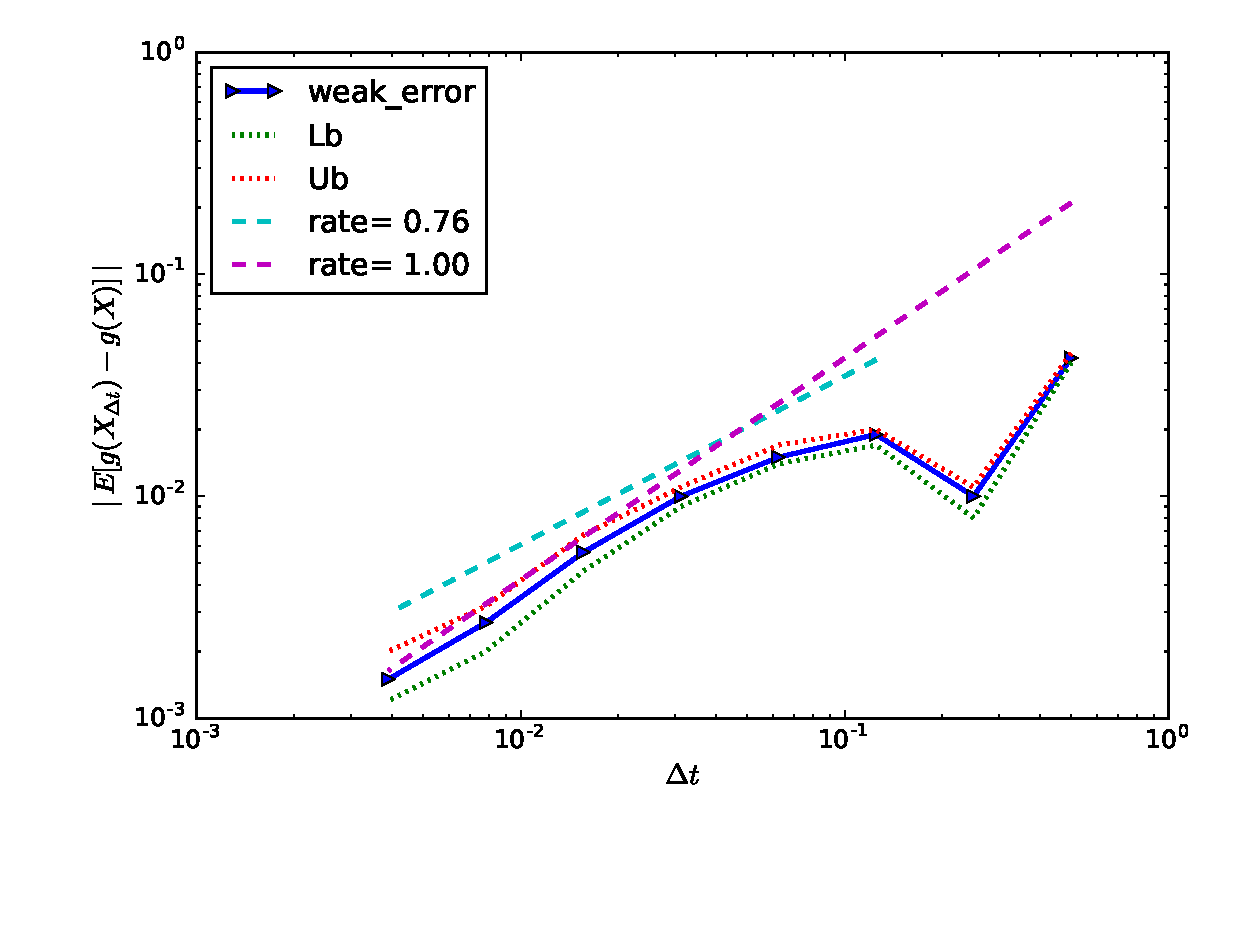
\includegraphics[width=1\linewidth]{./rBergomi_weak_error_cholesky/weak_convergence_order_Bergomi_H_007_K_1_M_4_10_6_CI_relative_cholesky_non_hierarchical_non_parallel_asymptotic}
		\caption{}
		\label{fig:set1_weak_rate_exact}
	\end{subfigure}
	\label{fig:Weak_rate_set1_set_2_without_rich_hyb+chol}
\end{figure}
\end{frame}




\begin{frame}[plain, shrink=4]\frametitle{\centerline{Hybrid scheme \cite{bennedsen2017hybrid}}}
\begin{small}
\begin{align*}
	\widetilde{W}_t^{\blue{H}} &= \int_0^t K^{\blue{H}}(t-s) dW_s^1, \quad t \ge 0, \\ 	K^{\blue{H}}(t-s) &= \sqrt{2\blue{H}} (t-s)^{\blue{H} - 1/2},\quad \forall \: 0 \le s \le t. 
	\end{align*}
	\end{small}
\begin{itemize}
\item 	The hybrid scheme \red{discretizes} the  $\widetilde{W}^\blue{H}$ process into \red{Wiener integrals of power functions and a Riemann sum}, appearing from approximating the kernel by power functions near the origin and step functions elsewhere.
\begin{small}
\begin{align*}
\widetilde{W}^H_{\frac{i}{N}} \approx \overline{W}^H_{\frac{i}{N}}&= \sqrt{2H} \left(  W^2_i+\sum_{k=2}^{i} \left(\frac{b_k}{N}\right)^{H-\frac{1}{2}} \left(W_{\frac{i-(k-1)}{N}}^1-W_{\frac{i-k}{N}}^1\right)\right)\COMMA
\end{align*}
\end{small}
\begin{itemize}
\item $N$ is the number of time steps 
\item $\{W^{2}_j\}_{j=1}^N$: \red{Artificially introduced} $N$ Gaussian random variables that are used for left-rule points in the hybrid scheme.
\item $b_k=\left(\frac{k^{H+\frac{1}{2}}-(k-1)^{H+\frac{1}{2} }}{H+\frac{1}{2}}\right)^{\frac{1}{H-\frac{1}{2}}}.$
\end{itemize}
\end{itemize}
\end{frame}





\section{Our Hierarchical Deterministic Quadrature Methods}
\frame[plain,noframenumbering]{\tableofcontents[currentsection,currentsubsection]}


\begin{frame}[plain,shrink=5]\frametitle{\centerline{Analytic smoothing}}
\begin{small}
\begin{align}\label{BS_formula_rbergomi}
C_{RB}\left( T, K \right) &= E\left[ \left(S_T - K \right)^+ \right]  \nonumber\\
&=\expt{\expt{(S_T-K)^+ \mid \sigma(W^1(t) ,t \le T)}}\nonumber \\
&=E\left[C_{BS}\left( \blue{S_0} = \operatorname{exp}\left(\rho \int_0^T \sqrt{v_t} dW_t^1 - \frac{1}{2}
\rho^2 \int_0^T v_t dt\right), \right. \right.\nonumber\\
&\quad \quad \quad \left.\left.\ \blue{k} = K , \ \blue{\sigma^2} = (1-\rho^2)
\int_0^T v_t dt \right) \right]\nonumber\\
&\approx \int_{\rset^{2\red{N}}} C_{BS} \left(\blue{G}(\mathbf{w}^{(1)},\mathbf{w}^{(2)})\right) \rho_{\red{N}}(\mathbf{w}^{(1)})  \rho_{\red{N}}(\mathbf{w}^{(2)}) d\mathbf{w}^{(1)} d\mathbf{w}^{(2)}\nonumber\\
&=C_{RB}^N \PERIOD
\end{align}
\end{small}
\begin{itemize}
\item $C_{\text{BS}}(\blue{S_0},\blue{k},\blue{\sigma^2})$: the Black-Scholes call price, for initial spot price $\blue{S_0}$, strike price $\blue{k}$, and volatility $\blue{\sigma^2}$.
\item \blue{$G$} maps $2N$ independent standard Gaussian random inputs to the parameters fed to Black-Scholes formula.
\item $\rho_{\red{N}}$: the multivariate Gaussian density, $\red{N}$: number of time steps.
\end{itemize} 
\end{frame}


\begin{frame}[plain,shrink=1]	
	\frametitle{\centerline{ Numerical integration methods}}

	\begin{itemize}
	\item \textbf{Plain Monte Carlo (MC)}
	\begin{itemize}
	\item $\red{\varepsilon(M)}=\Ordo{\red{M}^{-1/2}}$ 
	\item $(+)$ insensitive to $\blue{d}$, $(-)$ slow convergence,  no profit from regularity.
\end{itemize}	  
	\item \textbf{\red{Classical Quasi-Monte Carlo (QMC)}}
	\begin{itemize}
	\item $\red{\varepsilon(M)}=\Ordo{\red{M}^{-1}\log(\red{M})^{\blue{d}-1}}$ 
	\item  $(+)$ better convergence, $(-)$ sensitive to $\blue{d}$, no profit from regularity.
\end{itemize}	  
	\item \textbf{Quadrature based on product approaches} 
	\begin{itemize}
	\item $\red{\varepsilon(M)}=\Ordo{\red{M}^{-\blue{r}/\blue{d}}}$
	 \item $(+)$ profits from regularity, faster than QMC if $\blue{r}>\blue{d}$, $(-)$ highly sensitive to $\blue{d}$.
	\end{itemize}
	\item \red{\textbf{Sparse grids quadrature (SGQ)}}
	\begin{itemize}
	\item  $\red{\varepsilon(M)}=\Ordo{\red{M}^{-\blue{s}} \log(\red{M})^{(\blue{d}-1)(\blue{s}+1)}}$
	\item 	 $(+)$ profits from regularity, faster than QMC if $\blue{s}>1$, less sensitive to $\blue{d}$.
\end{itemize}	
\end{itemize}	 
	
$\red{\varepsilon}$: prescribed accuracy,  $\red{M}$: the amount of
work,  $\blue{d}$: dimension of problem, $\blue{r, s}$: smoothness indices (bounded mixed (total) derivatives up to order $\blue{s(r)}$).
\end{frame}




\begin{frame}[plain]	
	\frametitle{\centerline{Sparse grids I}}

\textbf{\blue{Goal:}} Given  $F: \rset^d \rightarrow \rset$ and a multi-index $\boldsymbol{\beta} \in \mathbb{N}^d_{+}$, \red{approximate}
\begin{displaymath} \expt{F} \approx Q^{m(\boldsymbol{\beta})}[F], \end{displaymath} 
where $Q^{m(\boldsymbol{\beta})}$ a Cartesian quadrature grid with $m(\beta_n)$ points along $y_n$.


\textbf{\blue{Idea:}} Denote $Q^{m(\boldsymbol{\beta})}[F]=F_{\boldsymbol{\beta}}$ and introduce the \red{first difference operator} 

\begin{equation*}
\begin{aligned}
\Delta_i F_{\boldsymbol{\beta}} \left\{ \begin{array}{rcr}
F_{\boldsymbol{\beta}} - F_{\boldsymbol{\beta}-e_i}, & \text{ if } \beta_i>1  \\ 
F_{\boldsymbol{\beta}}  & \text{ if } \beta_i=1  \end{array} \right. \\
\end{aligned}
\end{equation*}

where $e_i$ denotes the $i$th $d$-dimensional unit vector, and \red{mixed difference operators}

\begin{equation*}
\Delta [F_{\boldsymbol{\beta}}]= \otimes_{i = 1}^{d} \Delta_iF_{\boldsymbol{\beta}}
\end{equation*}

\end{frame}


\begin{frame}[plain,shrink=4]	
	\frametitle{\centerline{Sparse grids II}}
	\vspace{0.3cm}
 A quadrature estimate of $E[F]$ is
\begin{small}
\begin{equation}\label{eq:Quadrature_estimator}
\mathcal{M}_{\mathcal{I_{\ell}}}[F]=\sum_{\boldsymbol{\beta} \in \mathcal{I}_{\ell}} \Delta [F_{\boldsymbol{\beta}}]\COMMA
\end{equation}
\end{small}
\begin{itemize}
\item \red{Product approach}: $\mathcal{I}_{\ell}=\{ \max\{\beta_1,\dots,\beta_d \} \le \ell;\: \boldsymbol{\beta} \in \mathbb{N}^d_{+} \} $
\item \red{Regular SG}: $ \mathcal{I}_{\ell}=\{  \mid \boldsymbol{\beta} \mid_1 \le \ell+d-1; \: \boldsymbol{\beta} \in \mathbb{N}^d_{+} \} $

		\begin{figure}
		\centering
		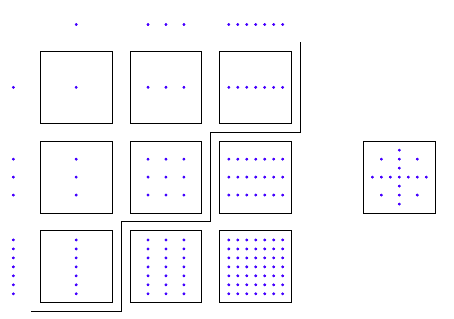
\includegraphics[scale=0.3]{sparse_grids}
%		\vspace{0.1cm}
		\caption{Left are product grids $\Delta_{\beta_1} \otimes \Delta_{\beta_2}$ for $1 \le \beta_1, \beta_2 \le 3$. Right is the corresponding SG construction.}
		\label{fig:vol_rough}
	\end{figure}
	\vspace{0.5cm}
\item \red{ASGQ}: $\mathcal{I}_{\ell}=\blue{\mathcal{I}^{\text{ASGQ}}}$.
\end{itemize}
\end{frame}

\begin{frame}[plain,shrink=2]	
	\frametitle{\centerline{ ASGQ in practice }}
	\vspace{0.2cm}
	\begin{itemize}
		\item The construction of \blue{$\mathcal{I}^{\text{ASGQ}}$} is done by \red{profit thresholding}
 \begin{equation*}
 \blue{\mathcal{I}^{\text{ASGQ}}}=\{\boldsymbol{\beta} \in \mathbb{N}^d_{+}: \blue{P_{\boldsymbol{\beta}}}	 \ge \overline{T}\}.
 \end{equation*}
 \item \textbf{Profit of a hierarchical surplus} \blue{$P_{\boldsymbol{\beta}}= \frac{\abs{\Delta E_{\boldsymbol{\beta}}}}{\Delta\mathcal{W}_{\boldsymbol{\beta}}}$}.
\item \textbf{Error contribution}:  \blue{ $\Delta E_{\boldsymbol{\beta}} = \abs{\mathcal{M}^{\mathcal{I} \cup \{\boldsymbol{\beta}\}}-\mathcal{M}^{\mathcal{I}}}$}.
%how much the error decreases if the operator $\Delta[F_{\boldsymbol{\beta}}]$ is added to \blue{$\mathcal{M}_{\mathcal{I}}[F]$
		\item \textbf{Work contribution}:  \blue{$ 		\Delta \mathcal{W}_{\boldsymbol{\beta}} = \text{Work}[\mathcal{M}^{\mathcal{I} \cup \{\boldsymbol{\beta}\}}]-\text{Work}[\mathcal{M}^{\mathcal{I}}]$}.	
		\begin{figure}
		\centering
		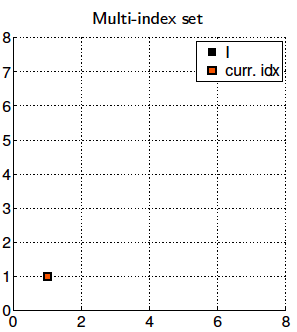
\includegraphics[scale=0.3]{./MISC_construction/1}
		\caption{\red{A posteriori, adaptive construction}: Given an index set $\mathcal{I}_k$, compute the profits of the neighbor indices and select the most profitable one}
	\end{figure}
		\end{itemize}
		
\end{frame}

\begin{frame}[plain,shrink=2,noframenumbering]	
	\frametitle{\centerline{ ASGQ in practice }}
	\vspace{0.2cm}
	\begin{itemize}
		\item The construction of \blue{$\mathcal{I}^{\text{ASGQ}}$} is done by \red{profit thresholding}
 \begin{equation*}
 \blue{\mathcal{I}^{\text{ASGQ}}}=\{\boldsymbol{\beta} \in \mathbb{N}^d_{+}: \blue{P_{\boldsymbol{\beta}}}	 \ge \overline{T}\}.
 \end{equation*}
 \item \textbf{Profit of a hierarchical surplus} \blue{$P_{\boldsymbol{\beta}}= \frac{\abs{\Delta E_{\boldsymbol{\beta}}}}{\Delta\mathcal{W}_{\boldsymbol{\beta}}}$}.
\item \textbf{Error contribution}:  \blue{ $\Delta E_{\boldsymbol{\beta}} = \abs{\mathcal{M}^{\mathcal{I} \cup \{\boldsymbol{\beta}\}}-\mathcal{M}^{\mathcal{I}}}$}.
%how much the error decreases if the operator $\Delta[F_{\boldsymbol{\beta}}]$ is added to \blue{$\mathcal{M}_{\mathcal{I}}[F]$
		\item \textbf{Work contribution}:  \blue{$ 		\Delta \mathcal{W}_{\boldsymbol{\beta}} = \text{Work}[\mathcal{M}^{\mathcal{I} \cup \{\boldsymbol{\beta}\}}]-\text{Work}[\mathcal{M}^{\mathcal{I}}]$}.	
		\begin{figure}
		\centering
		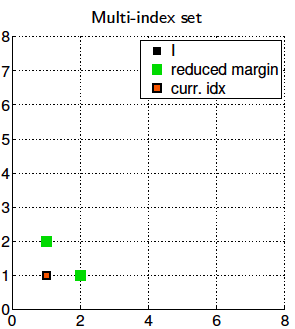
\includegraphics[scale=0.3]{./MISC_construction/2}
		\caption{\red{A posteriori, adaptive construction}: Given an index set $\mathcal{I}_k$, compute the profits of the neighbor indices and select the most profitable one.}
	\end{figure}
			\end{itemize}
\end{frame}

\begin{frame}[plain,shrink=2,noframenumbering]	
	\frametitle{\centerline{ ASGQ in practice }}
	\vspace{0.2cm}
	\begin{itemize}
		\item The construction of \blue{$\mathcal{I}^{\text{ASGQ}}$} is done by \red{profit thresholding}
 \begin{equation*}
 \blue{\mathcal{I}^{\text{ASGQ}}}=\{\boldsymbol{\beta} \in \mathbb{N}^d_{+}: \blue{P_{\boldsymbol{\beta}}}	 \ge \overline{T}\}.
 \end{equation*}
 \item \textbf{Profit of a hierarchical surplus} \blue{$P_{\boldsymbol{\beta}}= \frac{\abs{\Delta E_{\boldsymbol{\beta}}}}{\Delta\mathcal{W}_{\boldsymbol{\beta}}}$}.
\item \textbf{Error contribution}:  \blue{ $\Delta E_{\boldsymbol{\beta}} = \abs{\mathcal{M}^{\mathcal{I} \cup \{\boldsymbol{\beta}\}}-\mathcal{M}^{\mathcal{I}}}$}.
%how much the error decreases if the operator $\Delta[F_{\boldsymbol{\beta}}]$ is added to \blue{$\mathcal{M}_{\mathcal{I}}[F]$
		\item \textbf{Work contribution}:  \blue{$ 		\Delta \mathcal{W}_{\boldsymbol{\beta}} = \text{Work}[\mathcal{M}^{\mathcal{I} \cup \{\boldsymbol{\beta}\}}]-\text{Work}[\mathcal{M}^{\mathcal{I}}]$}.
		\begin{figure}
		\centering
		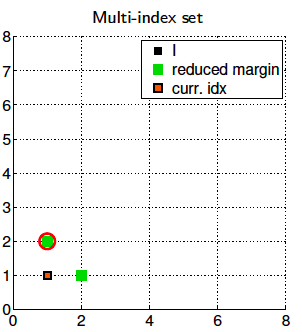
\includegraphics[scale=0.3]{./MISC_construction/3}
		\caption{\red{A posteriori, adaptive construction}: Given an index set $\mathcal{I}_k$, compute the profits of the neighbor indices and select the most profitable one.}
	\end{figure}
	\end{itemize}
\end{frame}
\begin{frame}[plain,shrink=2,noframenumbering]	
	\frametitle{\centerline{ ASGQ in practice }}
	\vspace{0.2cm}
	\begin{itemize}
		\item The construction of \blue{$\mathcal{I}^{\text{ASGQ}}$} is done by \red{profit thresholding}
 \begin{equation*}
 \blue{\mathcal{I}^{\text{ASGQ}}}=\{\boldsymbol{\beta} \in \mathbb{N}^d_{+}: \blue{P_{\boldsymbol{\beta}}}	 \ge \overline{T}\}.
 \end{equation*}
 \item \textbf{Profit of a hierarchical surplus} \blue{$P_{\boldsymbol{\beta}}= \frac{\abs{\Delta E_{\boldsymbol{\beta}}}}{\Delta\mathcal{W}_{\boldsymbol{\beta}}}$}.
\item \textbf{Error contribution}:  \blue{ $\Delta E_{\boldsymbol{\beta}} = \abs{\mathcal{M}^{\mathcal{I} \cup \{\boldsymbol{\beta}\}}-\mathcal{M}^{\mathcal{I}}}$}.
%how much the error decreases if the operator $\Delta[F_{\boldsymbol{\beta}}]$ is added to \blue{$\mathcal{M}_{\mathcal{I}}[F]$
		\item \textbf{Work contribution}:  \blue{$ 		\Delta \mathcal{W}_{\boldsymbol{\beta}} = \text{Work}[\mathcal{M}^{\mathcal{I} \cup \{\boldsymbol{\beta}\}}]-\text{Work}[\mathcal{M}^{\mathcal{I}}]$}.
		\begin{figure}
		\centering
		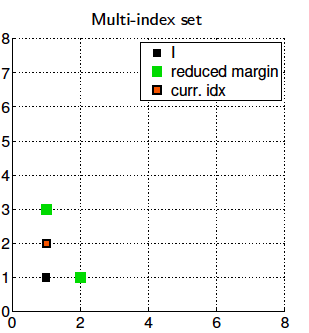
\includegraphics[scale=0.3]{./MISC_construction/4}
		\caption{\red{A posteriori, adaptive construction}: Given an index set $\mathcal{I}_k$, compute the profits of the neighbor indices and select the most profitable one.}
	\end{figure}
	\end{itemize}
\end{frame}

\begin{frame}[plain,shrink=2,noframenumbering]	
	\frametitle{\centerline{ ASGQ in practice }}
	\vspace{0.2cm}
	\begin{itemize}
		\item The construction of \blue{$\mathcal{I}^{\text{ASGQ}}$} is done by \red{profit thresholding}
 \begin{equation*}
 \blue{\mathcal{I}^{\text{ASGQ}}}=\{\boldsymbol{\beta} \in \mathbb{N}^d_{+}: \blue{P_{\boldsymbol{\beta}}}	 \ge \overline{T}\}.
 \end{equation*}
 \item \textbf{Profit of a hierarchical surplus} \blue{$P_{\boldsymbol{\beta}}= \frac{\abs{\Delta E_{\boldsymbol{\beta}}}}{\Delta\mathcal{W}_{\boldsymbol{\beta}}}$}.
\item \textbf{Error contribution}:  \blue{ $\Delta E_{\boldsymbol{\beta}} = \abs{\mathcal{M}^{\mathcal{I} \cup \{\boldsymbol{\beta}\}}-\mathcal{M}^{\mathcal{I}}}$}.
%how much the error decreases if the operator $\Delta[F_{\boldsymbol{\beta}}]$ is added to \blue{$\mathcal{M}_{\mathcal{I}}[F]$
		\item \textbf{Work contribution}:  \blue{$ 		\Delta \mathcal{W}_{\boldsymbol{\beta}} = \text{Work}[\mathcal{M}^{\mathcal{I} \cup \{\boldsymbol{\beta}\}}]-\text{Work}[\mathcal{M}^{\mathcal{I}}]$}.
		\begin{figure}
		\centering
		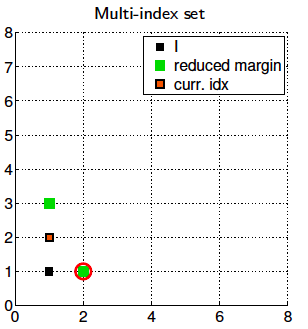
\includegraphics[scale=0.3]{./MISC_construction/5}
		\caption{\red{A posteriori, adaptive construction}: Given an index set $\mathcal{I}_k$, compute the profits of the neighbor indices and select the most profitable one.}
	\end{figure}
			
	\end{itemize}
\end{frame}

\begin{frame}[plain,shrink=2,noframenumbering]	
	\frametitle{\centerline{ ASGQ in practice }}
	\vspace{0.2cm}
	\begin{itemize}
		\item The construction of \blue{$\mathcal{I}^{\text{ASGQ}}$} is done by \red{profit thresholding}
 \begin{equation*}
 \blue{\mathcal{I}^{\text{ASGQ}}}=\{\boldsymbol{\beta} \in \mathbb{N}^d_{+}: \blue{P_{\boldsymbol{\beta}}}	 \ge \overline{T}\}.
 \end{equation*}
 \item \textbf{Profit of a hierarchical surplus} \blue{$P_{\boldsymbol{\beta}}= \frac{\abs{\Delta E_{\boldsymbol{\beta}}}}{\Delta\mathcal{W}_{\boldsymbol{\beta}}}$}.
\item \textbf{Error contribution}:  \blue{ $\Delta E_{\boldsymbol{\beta}} = \abs{\mathcal{M}^{\mathcal{I} \cup \{\boldsymbol{\beta}\}}-\mathcal{M}^{\mathcal{I}}}$}.
%how much the error decreases if the operator $\Delta[F_{\boldsymbol{\beta}}]$ is added to \blue{$\mathcal{M}_{\mathcal{I}}[F]$
		\item \textbf{Work contribution}:  \blue{$ 		\Delta \mathcal{W}_{\boldsymbol{\beta}} = \text{Work}[\mathcal{M}^{\mathcal{I} \cup \{\boldsymbol{\beta}\}}]-\text{Work}[\mathcal{M}^{\mathcal{I}}]$}.	
		\begin{figure}
		\centering
		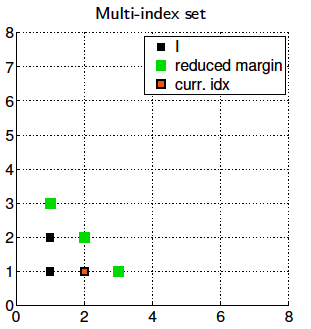
\includegraphics[scale=0.3]{./MISC_construction/6}
		\caption{\red{A posteriori, adaptive construction}: Given an index set $\mathcal{I}_k$, compute the profits of the neighbor indices and select the most profitable one.}
	\end{figure}

	
	\end{itemize}
\end{frame}

\begin{frame}[plain,shrink=2,noframenumbering]	
	\frametitle{\centerline{ ASGQ in practice }}
	\vspace{0.2cm}
	\begin{itemize}
		\item The construction of \blue{$\mathcal{I}^{\text{ASGQ}}$} is done by \red{profit thresholding}
 \begin{equation*}
 \blue{\mathcal{I}^{\text{ASGQ}}}=\{\boldsymbol{\beta} \in \mathbb{N}^d_{+}: \blue{P_{\boldsymbol{\beta}}}	 \ge \overline{T}\}.
 \end{equation*}
 \item \textbf{Profit of a hierarchical surplus} \blue{$P_{\boldsymbol{\beta}}= \frac{\abs{\Delta E_{\boldsymbol{\beta}}}}{\Delta\mathcal{W}_{\boldsymbol{\beta}}}$}.
\item \textbf{Error contribution}:  \blue{ $\Delta E_{\boldsymbol{\beta}} = \abs{\mathcal{M}^{\mathcal{I} \cup \{\boldsymbol{\beta}\}}-\mathcal{M}^{\mathcal{I}}}$}.
%how much the error decreases if the operator $\Delta[F_{\boldsymbol{\beta}}]$ is added to \blue{$\mathcal{M}_{\mathcal{I}}[F]$
		\item \textbf{Work contribution}:  \blue{$ 		\Delta \mathcal{W}_{\boldsymbol{\beta}} = \text{Work}[\mathcal{M}^{\mathcal{I} \cup \{\boldsymbol{\beta}\}}]-\text{Work}[\mathcal{M}^{\mathcal{I}}]$}.	
		\begin{figure}
		\centering
		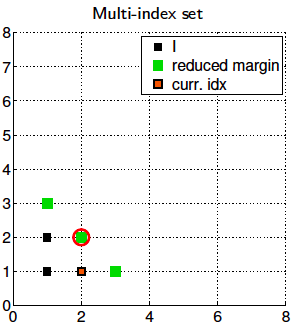
\includegraphics[scale=0.3]{./MISC_construction/7}
		\caption{ \red{A posteriori, adaptive construction}: Given an index set $\mathcal{I}_k$, compute the profits of the neighbor indices and select the most profitable one.}
	\end{figure}
	\end{itemize}
\end{frame}


\begin{frame}[plain, shrink=4]\frametitle{\centerline{Randomized QMC} }  
\begin{itemize}

\item \red{A (rank-$1$) lattice rule} \cite{sloan1985lattice,nuyens2014construction} with $n$ points 
\begin{equation*}
Q_n(f):=\frac{1}{n}\sum_{k=0}^{n-1} f \left( \frac{kz \: \text{mod}\: n}{n}\right),
\end{equation*}
where  $z = (z_1,\dots, z_d) \in \nset^d$.

\item \red{A randomly shifted lattice rule} 
\begin{align}
\overline{Q}_{n,q}(f)=\frac{1}{q} \sum_{i=0}^{q-1}Q^{(i )}_n(f)=\frac{1}{q}\sum_{i=0}^{q-1}\left(\frac{1}{n}\sum_{k=0}^{n-1} f \left( \frac{kz+\Delta^{(i)}  \: \text{mod}\: n}{n}\right)  \right),
\end{align}
where $\{\Delta^{(i)}\}_{i=1}^q$: independent random shifts, and $M^{\text{QMC}}=q \times n$.

\begin{itemize}
\item  Unbiased approximation of the integral.
\item  Practical error estimate.
\end{itemize}
\item We use a pre-made point generators using latticeseq\_b2.py from   \url{https://people.cs.kuleuven.be/~dirk.nuyens/qmc-generators/}.
\end{itemize}

\end{frame}



\begin{frame}[plain,shrink=8]\frametitle{\centerline{Path generation methods} }  
$\{t_i\}_{i=0}^{N}$: Grid of time steps, $\{B_{t_i}\}_{i=0}^{N}$: Brownian motion increments 
		\begin{itemize}
			\item \textbf{\red{Random Walk}}
			\begin{itemize}
				\item Proceeds incrementally, given $B_{t_i}$,
					\begin{equation*}
				B_{t_{i+1}}=B_{t_i}+ \sqrt{\Delta t} z_i, \: z_i \sim \mathcal{N}(0,1) \PERIOD
				\end{equation*}
				\item All components of $\mathbf{z} = (z_1,\dots,z_N)$ have the same scale of importance: \red{isotropic}.
			\end{itemize}
			\item \textbf{\red{Hierarchical Brownian Bridge}} \cite{glasserman2004monte}
			\begin{itemize}
				\item Given a past value $B_{t_i}$ and a future value $B_{t_k}$, the value $B_{t_j}$ (with $t_i < t_j < t_k$) can be generated according to ($\rho=\frac{j-i}{k-i}$)
				\begin{equation}\label{eq: Brownian Bridge construction}
				B_{t_j}=(1-\rho) B_{t_i}+\rho B_{t_k}+ \sqrt{\rho (1-\rho)(k-i) \Delta t} z_j, \: z_j \sim \mathcal{N}(0,1) \PERIOD
				\end{equation}
					\item The most important values (determine the large scale structure of Brownian motion) are the first components of $\mathbf{z} = (z_1,\dots,z_N)$.
					\item $\searrow$ the \red{effective dimension} ($\#$ important dimensions) and $\nearrow$  \red{anisotropy} between different directions $\Rightarrow$ \red{Faster} ASGQ and QMC convergence.
			\end{itemize} 
		
	\end{itemize}
\end{frame}


\begin{frame}[plain, shrink=2]\frametitle{\centerline{Error comparison}}
\vspace{0.2cm}
$\red{\mathcal{E}_{\text{tot}}}$: the total error of approximating the  expectation in \eqref{BS_formula_rbergomi}.
\begin{itemize}
	\item When using ASGQ estimator, $Q_N$
	\begin{align*}
	\red{\mathcal{E}_{\text{tot}}} & \le \abs{C_{\text{RB}}-C_{\text{RB}}^N}+\abs{C_{\text{RB}}^N-Q_{N}} \le \green{\mathcal{E}_B(N)}+ \blue{\mathcal{E}_Q(\text{TOL}_{\text{ASGQ}},N)},
	\end{align*}
where  $\mathcal{E}_Q$ is the quadrature error, $\green{\mathcal{E}_B}$  is the bias, $\blue{\text{TOL}_{\text{ASGQ}}}$ is a user selected tolerance for ASGQ method.
\item When using randomized QMC or MC estimator,   $Q^{\text{MC (QMC)}}_N$
		\begin{align*}
	\red{\mathcal{E}_{\text{tot}}} & \le \abs{C_{\text{RB}}-C_{\text{RB}}^N}+\abs{C_{\text{RB}}^N-Q^{\text{MC (QMC)}}_N} \le \green{\mathcal{E}_B(N)}+ \blue{\mathcal{E}_{S}(M,N)},
	\end{align*}
	where  $\blue{\mathcal{E}_S}$ is the statistical error, $\blue{M}$ is the number of samples used for MC or randomized QMC method.
	\item $\blue{M^{\text{QMC}}}$ and $\blue{M^{\text{MC}}}$, are chosen so that $\blue{\mathcal{E}_{S,\text{QMC}}(M^{\text{QMC}})}$ and  \blue{$\mathcal{E}_{S,\text{MC}}(M^{\text{MC}})$} satisfy
	\begin{align*}
	\blue{\mathcal{E}_{S,\text{QMC}}(M^{\text{QMC}})}=\blue{\mathcal{E}_{S,\text{MC}}(M^{\text{MC}})}= \green{\mathcal{E}_B(N)}=\frac{\red{\mathcal{E}_{\text{tot}}}}{2}\PERIOD
	\end{align*}
\end{itemize}
\end{frame}


\section{Numerical Experiments and Results}
\frame[plain,noframenumbering]{\tableofcontents[currentsection,currentsubsection]}



\begin{frame}[plain]\frametitle{\centerline{Numerical experiments}}
\vspace{0.1cm}
\begin{table}[!h]
\begin{tiny}
	\centering
\caption{Reference solution (using MC with $500$ time steps and number of samples, $M=8 \times 10^6$) of call option price under the rough Bergomi model, for different parameter constellations.  The numbers between parentheses correspond to the statistical errors estimates.}
\label{table:Reference solution, using MC with $500$ time steps, of Call option price under rBergomi model, for different parameter constellation.}
	\begin{tabular}{l*{2}{c}r}
	\toprule[1.5pt]
		\textbf{Parameters}            & \textbf{Reference solution}    \\
	\hline
		
		Set $1$:	$H=0.07, K=1,S_0=1, T=1, \rho=-0.9, \eta=1.9,\xi_0=0.235^2$   & $\underset{(5.6e-05)}{0.0791}$  \\	
		
		Set $2$:	$H=0.02, K=1, S_0=1, T=1,\rho=-0.7, \eta=0.4,\xi_0=0.1$   & $\underset{(9.0e-05)}{0.1246}$  \\
		Set $3$:	$H=0.02, K=0.8,S_0=1,T=1, \rho=-0.7, \eta=0.4,\xi_0=0.1$   & $\underset{(5.4e-05)}{0.2412}$  \\
		Set $4$:	$H=0.02, K=1.2,S_0=1,T=1, \rho=-0.7, \eta=0.4,\xi_0=0.1$   & $\underset{(8.0e-05)}{0.0570}$  \\
	\bottomrule[1.25pt]
	\end{tabular}
	\end{tiny}
\end{table}

\begin{itemize}
\item The first set is the  \red{closest to the empirical findings} \cite{gatheral2018volatility,bennedsen2016decoupling}, suggesting that $\blue{H} \approx 0.1$. The choice of values $\blue{\nu}= 1.9$ and $\blue{\rho}=-0.9$ is justified by \cite{bayer2016pricing}.

\item  For the remaining three sets, we wanted to test the potential of our method for a \red{very rough case}, where variance reduction methods are inefficient.
\end{itemize}
\end{frame}
\begin{frame}[plain]\frametitle{\centerline{Relative errors and computational gains}}
\begin{table}[!h]
	\begin{tiny}
	\centering
	\caption{ In this table, we highlight the computational gains achieved by ASGQ and QMC over MC method to meet a certain error tolerance. We note that the ratios are computed \red{for the best configuration with Richardson extrapolation for each method}.}
		\begin{tabular}{l*{4}{c}r}
			\toprule[1.5pt]
			\textbf{Parameter set}              &  \textbf{Relative error}  & \textbf{CPU time ratio $\left(\text{MC}/ \text{ASGQ} \right)$} & \textbf{CPU time ratio  $\left(\text{MC}/ \text{QMC} \right)$}\\
			\hline
			Set $1$  &  $1\%$&  $ 15$ &  $10$\\	
			
			\hline
		Set $2$    &  $0.2\%$&  $21.5$ &  $73.2$\\		
			\hline
		Set $3$   &  $0.4\%$&  $26.7$ &  $21.3$\\	
			\hline
		Set $4$ &  $2\%$&  $5$ &  $10$\\	
			\bottomrule[1.25pt]
		\end{tabular}
	\label{table:Summary of our numerical results.}
		\end{tiny}
\end{table}
\end{frame}
\begin{frame}[plain]\frametitle{\centerline{Complexity of the different  methods}}

%\\ \centerline{with the Different Configurations}}
 
\begin{figure}
	\centering
	\begin{subfigure}{0.495\textwidth}
		\centering
		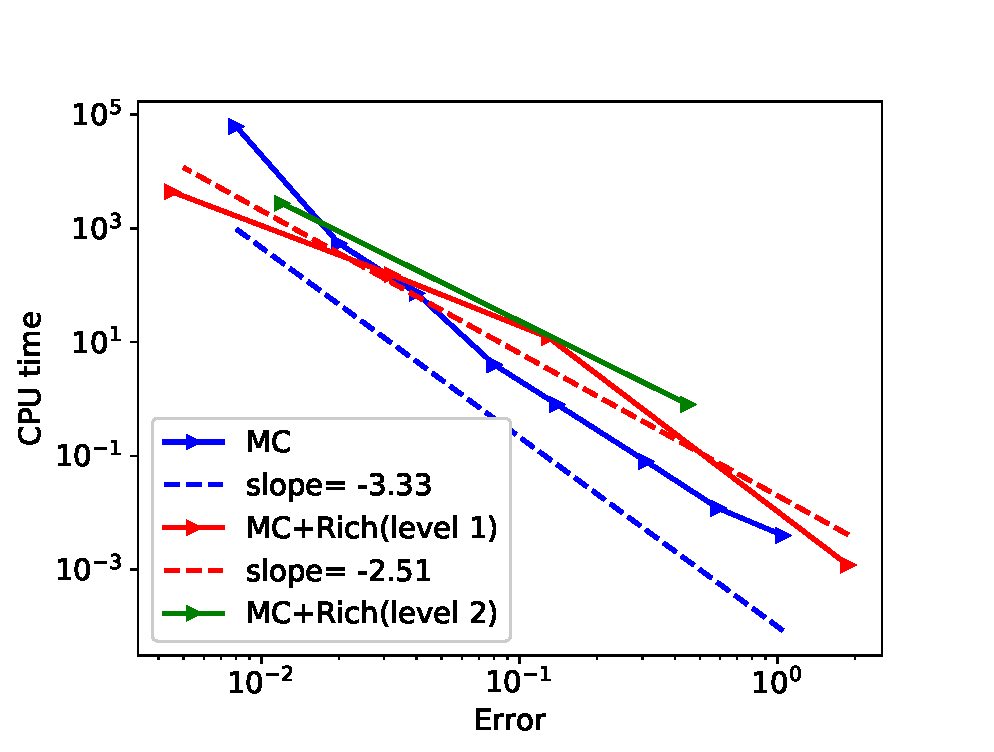
\includegraphics[width=0.6\textwidth]{./rBergomi_Complexity_rates/set2/error_vs_time_set2_MC_comparison}
		\caption{}
	\end{subfigure}
	\begin{subfigure}{0.495\textwidth}
		\centering
		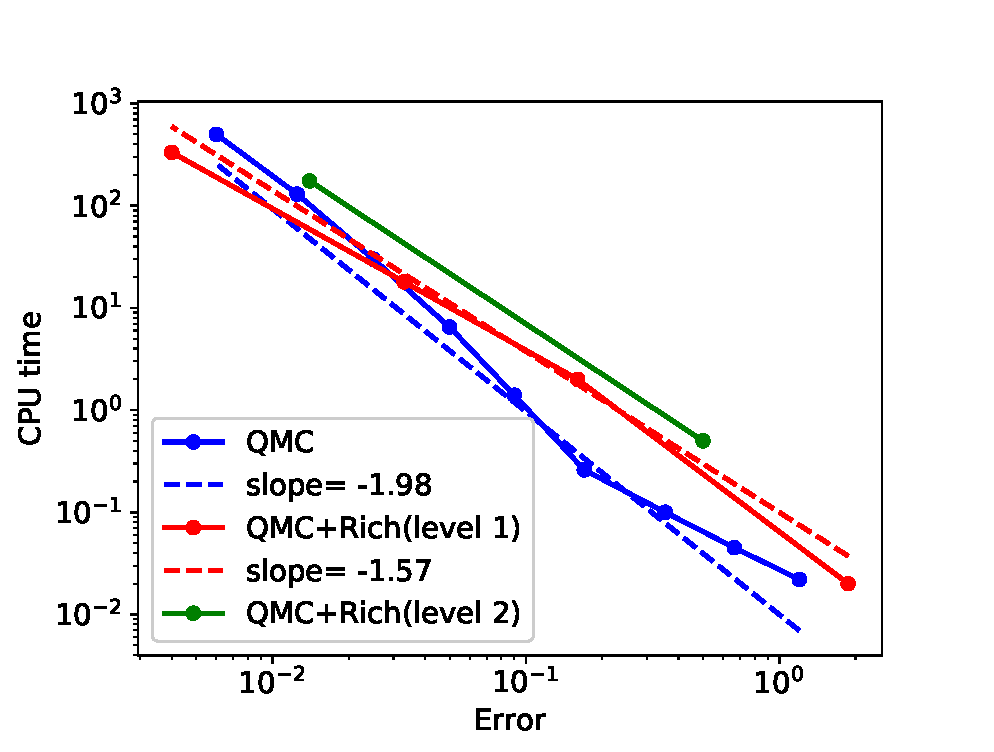
\includegraphics[width=0.6\textwidth]{./rBergomi_Complexity_rates/set2/error_vs_time_set2_QMC_comparison}
		\caption{}
	\end{subfigure}
	\begin{subfigure}{0.5\textwidth}
		\centering
		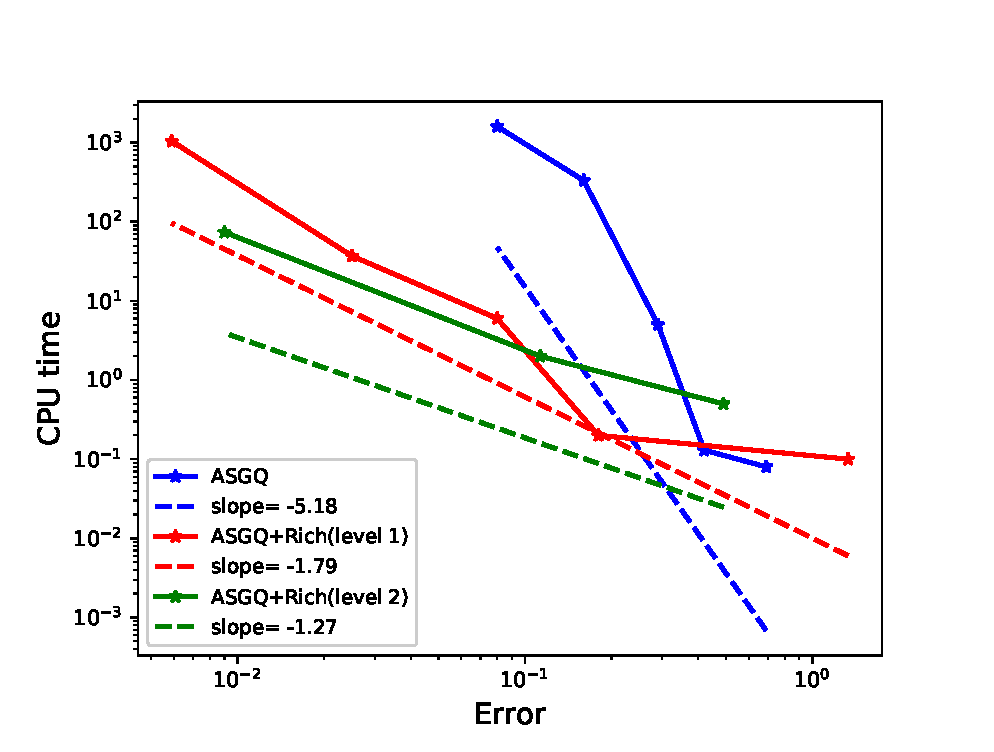
\includegraphics[width=0.6\textwidth]{./rBergomi_Complexity_rates/set2/error_vs_time_set2_MISC_comparison}
		\caption{}
	\end{subfigure}%%
	\caption{Numerical complexity of the different  methods with the different configurations in terms of  Richardson extrapolation 's level.  Case of \red{parameter set $1$ in Table \ref{table:Reference solution, using MC with $500$ time steps, of Call option price under rBergomi model, for different parameter constellation.}}. a) \red{MC methods}. b) \red{QMC methods}. d) \red{ASGQ methods}. }
	\label{fig: Comparing the numerical complexity of the different  methods with the different configurations}
\end{figure}
\end{frame}


\begin{frame}[plain]\frametitle{\centerline{Complexity of the different methods}\\
\centerline{with their best configurations}}
\begin{figure}[h!]
	\centering
	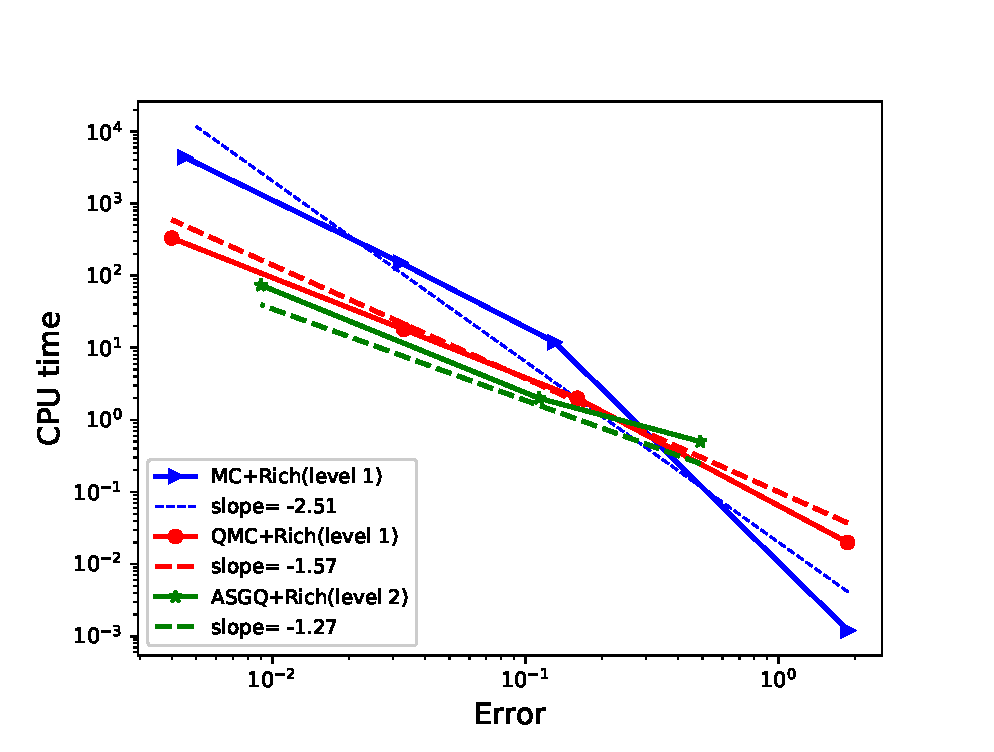
\includegraphics[width=0.6\linewidth]{./rBergomi_Complexity_rates/set2/error_vs_time_set2_full_comparison}
	\caption{Computational work comparison for the different methods \red{with the best configurations concluded from Figure \ref{fig: Comparing the numerical complexity of the different  methods with the different configurations}}, for the case of \red{parameter set $1$ in Table \ref{table:Reference solution, using MC with $500$ time steps, of Call option price under rBergomi model, for different parameter constellation.}}.}	\label{fig:Complexity plot for  MISC for Case set $2$ parameters, comparison}
\end{figure}
\end{frame}



%%%%%%%%%%%%%%%%%%%%%%%%%%%%%%%%%%%%%%%%%%%%%%%%%%%%%%%%%%%%%%%%%%%%%%%%%%%%%%%%%%%%%%%%%%%%%%%%%%%%%%%%%%%%%%%%%%%%%%%%%%%%
\section{Conclusions}
\frame[plain,noframenumbering]{\tableofcontents[currentsection,currentsubsection]}

\begin{frame}[plain]\frametitle{\centerline{Conclusions}}
\begin{itemize}
\item Proposed novel, \red{fast option pricers, based on hierarchical deterministic quadrature methods}, for options whose underlyings follow \red{the rBergomi model}.
\item Given a sufficiently small relative error tolerance, our proposed methods demonstrate \red{substantial computational gains over the standard MC method}, for different parameter constellations.
\item Accelerating our novel methods can be achieved by using  more optimal hierarchical path generation method than Brownian bridge construction, such as PCA or LT transformations.
\end{itemize}
\end{frame}

%%%%%%%%%%%%%%%%%%%%%%%%%%%%%%%%%%%%%%%%%%%%%%%%%%%%%%%%%%%%%%%%%%%%%%%%%%%%%%%%%%%%%%%%%%%%%%%%%%%%%%%%%%%%%%%%%%%%%%%%%%%%


%\section*{}
\begin{frame}[plain,,noframenumbering]
	\LARGE\begin{center}
		Thank you for your attention
	\end{center}
\end{frame}


%%%%%%%%%%%%%%%%%%%%%%%%%%%%%%%%%%%%%%%%%%%%%%%%%%%%%%%%%%%%

%\medskip
%\section{References}

\begin{frame}[plain,noframenumbering,allowframebreaks]
	\frametitle{References}
	\raggedright
	\nocite{*}
	\bibliographystyle{apalike}
	\bibliography{smoothing_rBergomi}
\end{frame}




%\begin{frame}[plain,shrink=10]
%	\frametitle{\centerline{The Stochastic Simulation Algorithm (SSA) }\\
%		\centerline{\cite{gillespie_ssa}}}
%	
%	
%	\begin{enumerate}
%		\item Initialize $\mathbf{x} \leftarrow \mathbf{x}_0$ (The initial number of molecules of each species)  and $ t \leftarrow 0$.
%		\item  In state $\mathbf{x}$ at time t, compute $(a_j(\mathbf{x}))_{j=1}^{J}$ and the sum
%		$a_0(\mathbf{x}) = \sum_{j=1}^{J}a_j (\mathbf{x})$.
%		
%		\item Generate two independent  uniform $(0,1)$ random number $r_1$ and $r_2$.
%		
%		\item Set (equivalent to generating an \red{exponential RV} with parameter $a_0$.)
%		\begin{align*}
%		\tau=\frac{1}{a_0} \operatorname{ln}(1/r_1)
%		\end{align*}
%		
%		
%		\red{Caveat}:  $\expt{\tau \mid \mathbf{X}(t)=\mathbf{x}}=\LP a_0(\mathbf{x})\RP^{-1}$ \red{could be very small}.
%		
%		\item Find $j \in \{1,\dots, J\}$  such that
%		\begin{align}
%		a_0^{-1} \sum_{k=1}^{j-1} a_j <r_2 \leq a_0^{-1}\sum_{k=1}^{j} a_j
%		\end{align}
%		which is equivalent  to choosing from reactions $\{1,\dots,J \}$ with the $j^{th}$ reaction having probability mass function $ \LP a_j (\mathbf{x})/a_0(\mathbf{x})\RP_{j=1}^{J}$.
%		
%		\item Update: $t \leftarrow  t + \tau$  and $ \mathbf{x} \leftarrow  \mathbf{x}+\boldsymbol{\nu}_{j}$.
%		\item Record $(t, \mathbf{x})$. Return to step $2$ if $t < T$, otherwise end the
%		simulation.
%		
%	\end{enumerate}
%\end{frame}
%
%
%%%%%%%%%%%%%%%%%%%%%%%%%%%%%%%%%%%%%%%%%%%%%%%%%%%%%
%
%\begin{frame}[plain,shrink=10]
%	\frametitle{\centerline{The Explicit-TL Method }\\
%		\centerline{\cite{gillespie_tau_leap,Aparicio_tau_leap}}}
%	\vspace{0.2cm}
%	We obtain the explicit-TL method (kind of forward Euler approximation): Given $ \mathbf{Z}^{\text{exp}} (t)=  \mathbf{z} \in \zset_+^d$,
%	\begin{equation*}\label{approx}
%	\mathbf{Z}^{exp} (t+\tau) =\mathbf{z}+\sum_{j=1}^{J} \mathcal{P}_{j} \LP \underbrace{a_{j}(\mathbf{z}) \tau}_{\lambda_j} \RP \boldsymbol{\nu}_{j} \COMMA
%	\end{equation*}
%	$\mathcal{P}_j (\lambda_j ) $ are independent Poisson random variables with rate $\lambda_j$.
%	
%	\red{Caveat}:  The explicit-TL is not adequate when dealing with \red{stiff problems} ( $\text{\color{red}  Numerical stability} \color{black} \Rightarrow \color{blue} \tau^{exp}_{threshold} \ll 1 \color{black} .$)
%\end{frame}
%
%\begin{frame}[plain]
%	
%	\frametitle{\centerline{Split Step Implicit Tau-Leap (SSI-TL) Method I} \\
%		\centerline{\cite{Chiheb_ML_implicit}}}
%	\vspace{0.2cm}
%	The  \red{\nameexp} scheme, where $\mathbf{z}=\mathbf{Z}^{exp} (t)$,  can be rewritten as follows:
%	\begin{align}\label{explicit2}
%	\mathbf{Z}^{exp} (t+\tau) &=\mathbf{z}+\sum_{j=1}^{J} \mathcal{P}_{j} \LP a_{j}(\mathbf{z}) \tau \RP \boldsymbol{\nu}_{j} \nonumber\\
%	&=\mathbf{z}+\sum_{j=1}^{J} \LP \mathcal{P}_{j} \LP a_{j}(\mathbf{z}) \tau \RP - a_{j}(\mathbf{z}) \tau + a_{j}(\mathbf{z}) \tau \RP  \boldsymbol{\nu}_{j} \nonumber\\
%	&=  \mathbf{z}+ \underbrace{ \sum_{j=1}^{J} a_{j}(\mathbf{z})  \tau  \boldsymbol{\nu}_{j}}_\text{\color{blue}drift} \color{black} + \underbrace{\sum_{j=1}^{J} \LP \mathcal{P}_{j} \LP a_{j}(\mathbf{z}) \tau \RP - a_{j}(\mathbf{z}) \tau \RP  \boldsymbol{\nu}_{j}}_\text{\color{red}zero-mean noise}\PERIOD
%	\end{align}
%	
%	%Let us denote the second and third quantities in the right-hand side of (\ref{explicit2}) by the drift and the zero-mean noise, respectively.
%\end{frame}
%
%
%\begin{frame}[plain]
%	\frametitle{\centerline{Split Step Implicit Tau-Leap (SSI-TL) Method II}}
%	\vspace{0.2cm}
%	The idea of \red{\name}  method is to take only the drift part as implicit while the noise part is left explicit. Let us define
%	$\mathbf{z}=\mathbf{Z}^{imp} (t)$ and define 
%	$\mathbf{Z}^{imp} (t+\tau)$ through the following  two steps:
%	\begin{align}\label{partial_implicit}
%	\mathbf{y} &= \mathbf{z}+\sum_{j=1}^{J}  a_{j} \LP \mathbf{y}\RP    \tau \boldsymbol{\nu}_{j}\text{ (\blue {Drift-Implicit step})}\\\nonumber
%	\mathbf{Z}^{imp} (t+\tau) &=  \mathbf{y} + \sum_{j=1}^{J} \LP \mathcal{P}_{j}(a_{j}(\mathbf{y}) \tau)-  a_{j}(\mathbf{y})\tau\RP   \boldsymbol{\nu}_{j}\\
%	\nonumber
%	&=  \mathbf{z} + \sum_{j=1}^{J}  \mathcal{P}_{j}(a_{j}(\mathbf{y}) \tau)   \boldsymbol{\nu}_{j}\text{ (\red {Tau-leap step})}\end{align}
%\end{frame}
%
%%%%%%%%%%%%%%%%%%%%%%%%%%%%%%%%%%%%%%%%%%%%%%%%%%%%%%%%%%%%%%%%%%%%%%%
%
%
%
%
%%%%%%%%%%%%%%%%%%%%%%%%%%%%%%%%%%%%%%%%%%%%%%%%%%%%%%%%%%%%%%%%%%%%%%%
%%\section{Multilevel Hybrid SSI-TL}
%%\frame{\tableofcontents[currentsection]}
%%\addtocounter{framenumber}{-1}
%%%%%%%%%%%%%%%%%%%%%%%%%%%%%%%%%%%%%%%%%%%%%%%%%%%%%%%%%%%%%%%%%%%%%%%
%
%
%
%
%\begin{frame}[plain,shrink=10]
%	
%	\frametitle{\centerline{Multilevel Hybrid SSI-TL I} \\
%		\centerline{\cite{Chiheb_ML_implicit}}}
%	\vspace{0.2cm}
%	Our multilevel hybrid SSI-TL  estimator is defined as:
%	
%	\begin{equation}\label{MLMCest_hybrid}
%	\hat{Q}:= \hat{Q}_{\red \Lc}+\sum\limits_{\ell=\red{\Lc}+1}^{\blue{\Li}-1} \hat{Q}_{\ell}+ \hat{Q}_{\blue \Li} +\sum\limits_{\ell=\blue{\Li}+1}^{\green L} \hat{Q}_{\ell}\COMMA
%	\end{equation}
%	
%	where 
%	\begin{align}\label{estimators_hybrid}
%	\begin{cases} 
%	\hat{Q}_{\red \Lc}:= \frac{1}{N_{i,\red \Lc}} \sum\limits_{n=1}^{N_{i,\red \Lc}} g(\mathbf{Z}^{imp}_{\red \Lc,[n]}(T)) \\ 
%	\hat{Q}_{\ell}:= \frac{1}{N_{ii,\ell}} \sum\limits_{n_{\ell}=1}^{N_{ii,\ell}}  \LP g(\mathbf{Z}^{imp}_{\ell,[n_{\ell}]}(T))-g(\mathbf{Z}^{imp}_{\ell-1,[n_{\ell}]}(T)) \RP, \: \:  \red{\Lc}+1 \leq \ell \leq  \blue{\Li}-1  \\
%	\hat{Q}_{\blue{\Li}}:= \frac{1}{N_{ie,\blue{\Li}}} \sum\limits_{n=1}^{N_{ie,\blue \Li}}  \LP g(\mathbf{Z}^{exp}_{\blue \Li,[n]}(T))-g(\mathbf{Z}^{imp}_{\blue{\Li}-1,[n]}(T)) \RP \\
%	\hat{Q}_{\ell}:= \frac{1}{N_{ee,\ell}} \sum\limits_{n_{\ell}=1}^{N_{ee,\ell}}  \LP g(\mathbf{Z}^{exp}_{\ell,[n_{\ell}]}(T))-g(\mathbf{Z}^{exp}_{\ell-1,[n_{\ell}]}(T)) \RP  , \: \:  \blue{\Li}+1 \leq \ell \leq  \green L  \PERIOD \\
%	\end{cases}
%	\end{align}
%\end{frame}
%
%
%\begin{frame}[plain,shrink=10]
%	\frametitle{\centerline{ Coupling (Idea)}\\
%		\centerline{\cite{Kurtz_coupling,Anderson2012} }}
%	\begin{itemize}
%		\item To couple two Poisson random variables, $\mathcal{P}_{1}(\lambda_{1} )$, $\mathcal{P}_{2}(\lambda_{2} )$, with rates $\lambda_{1}$ and $\lambda_{2}$, respectively, we define $ \color{blue} \lambda^{\star} \color{black}:=\operatorname{min} \{ \lambda_{1} ,\lambda_{2} \}$ and we consider the decomposition
%		\begin{align*}
%		\begin{cases} 
%		\mathcal{P}_{1} (\lambda_{1}):= \color{blue} \mathcal{Q}(\lambda^{\star})+ \color{black} \mathcal{Q}_{1}(\lambda_{1}-\color{blue} \lambda^{\star} \color{black}) \\ 
%		\mathcal{P}_{2} (\lambda_{2}):= \color{blue} \mathcal{Q}(\lambda^{\star}) \color{black}+ \mathcal{Q}_{2}(\lambda_{2}-\color{blue} \lambda^{\star} \color{black})
%		\end{cases}
%		\end{align*}
%		where $\mathcal{Q}(\color{blue} \lambda^{\star} \color{black})$, $\mathcal{Q}_{1}(\lambda_{1}-\color{blue} \lambda^{\star} \color{black})$ and $\mathcal{Q}_{2}(\lambda_{2}-\color{blue} \lambda^{\star} \color{black})$ are three independent Poisson random variables.
%		\item We have small variance between the coupled processes
%		\begin{small}
%			\begin{align*}
%			\var{\mathcal{P}_{1} (\lambda_{1})-\mathcal{P}_{2} (\lambda_{2})} &=\var{ \Big[ \mathcal{Q}_{1}(\lambda_{1}-\color{blue} \lambda^{\star} \color{black})-\mathcal{Q}_{2}(\lambda_{2}-\color{blue} \lambda^{\star} \color{black})\Big]} \\
%			&= \mid \lambda_{1} -\lambda_{2} \mid.
%			\end{align*}
%		\end{small}
%	\end{itemize}
%	\red{Observe}: If $\mathcal{P}_{1} (\lambda_{1})$ and $\mathcal{P}_{2} (\lambda_{2})$ are independent, then, we have a
%	larger variance $\var{\mathcal{P}_{1} (\lambda_{1})- \mathcal{P}_{2} (\lambda_{2})}=\lambda_{1}+\lambda_{2}.$
%\end{frame}
%
%
%
%\begin{frame}[plain,shrink=10]
%	\frametitle{\centerline{Multilevel Hybrid SSI-TL II}}
%	\vspace{2cm}
%	
%	\begin{equation}\label{MLMCest_hybrid}
%	\hat{Q}:= \hat{Q}_{\red \Lc}+\sum\limits_{\ell=\red{\Lc}+1}^{\blue{\Li}-1} \hat{Q}_{\ell}+ \hat{Q}_{\blue \Li} +\sum\limits_{\ell=\blue{\Li}+1}^{\green L} \hat{Q}_{\ell}\COMMA
%	\end{equation}
%	
%	\begin{enumerate}
%		\item $\red \Lc$, the coarsest discretization level.
%		\item $\blue \Li$, the interface level.
%		\item $\green L$, the finest discretization level.
%		\item $\mathbf{N} := \{N_{i,\red \Lc}, \{N_{ii,\ell}\}_{\ell=\red{\Lc}+1}^{\blue{\Li}-1},N_{ie,\blue{\Li}},\{ N_{ee,\ell}\}_{\ell=\blue{\Li}+1}^{\green L}\}$, the number of samples per level.
%	\end{enumerate}
%	
%	
%	
%\end{frame}



\end{document}